
\documentclass{llncs}
\usepackage{geometry}                
%\geometry{letterpaper}                   % ... or a4paper or a5paper or ... 
\usepackage{graphicx}
\usepackage{amssymb}
\usepackage{epstopdf}
\begin{document}

\title{Generating reliable service composition  using policies: a model-driven approach\thanks{This work is partially financed by the projects {\sc Orchestra} ECOS-ANUIES, {\sc e-CLOUDSS} Microsoft,  {\sc Clever} STIC-AMSUD, and {\sc Masai}.}}

\author{Genoveva Vargas-Solar\inst{1} 
\and Valeria de Castro\inst{4}
\and Pl\'{a}cido A. de Souza Neto\thanks{Financed by CAPES/SticAmbud Brasil, BEX 4112/11-3} \inst{5,6} 
\and Javier A. Espinosa-Oviedo\inst{3} 
\and Esperanza Marcos\inst{4} 
\and Mart\'{i}n A. Musicante\inst{5} 
\and Jos\'{e}-Luis Zechinelli-Martini\inst{2,1} 
\and Christine Collet \inst{3}}

\institute{
	French Council of Scientific Research, LIG-LAFMIA	\\
	681 Rue de la Passerelle, BP. 72, 38402	Saint Martin d'H\`{e}res Cedex, France		\\
		\email{Genoveva.Vargas-Solar@imag.fr}
\and
	Fundaci\'{o}n Universidad de las Am\'{e}ricas Puebla	\\
	Exhacienda Sta. Catarina M\'{a}rtir s/n 72820, San Andr\'{e}s Cholula, Puebla, M\'{e}xico			\\
	\email{joseluis.zechinelli@udlap.mx}
\and
	Grenoble Institute of Technology	\\
	46 Avenue F'{e}lix Viallet, 38031 Grenoble Cedex 1		\\
	\email{Christine.Collet@grenoble-inp.fr}, \email{Javier.Espinosa@imag.fr} \\
\and
	Universidad Rey Juan Carlos	\\
	Av Tulip\'{a}n, M\'{o}stoles, Spain 		\\
	\email{Valeria.deCastro@urjc.es, esperanza.marcos@urjc.es} \\
\and
	DIMAp - UFRN, ForAll - Formal Methods and Language Research Laboratory	\\
	Campus Universit�rio - Lagoa Nova, Natal - RN, Brasil		\\
	\email{mam@dimap.ufrn.br} \\
	\and
	Instituto Federal do Rio Grande do Norte	\\
	Av. Senador Salgador Filho, 1559 - Tirol, Natal - RN, Brasil		\\
	\email{placido.neto@ifrn.edu.br}
}

\maketitle

\begin{abstract}
This paper presents an approach for modeling and associating policies to  service based applications for representing both systems' cross-cutting aspects (e.g., exception handling expressing what to do when a service is not available, recovery, persistence) and  constraints stemming from the services used for implementing them (e.g., the fact that a service requires imposes an authentication protocol for executing a method).  Our work proposes a model driven  methodology that  (i) extends     PIM layer's composition model of the SOD-M method \cite{decastro1} with the notion of {\sf\small A-Policy} \cite{Espinosa-Oviedo2011a} for representing constraints associated to service based applications and, (ii) defines the $\pi$-{\sc Pews}  meta-model \cite{Placido2010LTPD} providing guidelines for expressing the composition and the policies (iii) defines   Model to model transformation rules for generating  the implementation of reliable services' compositions.
% (iv) defines model to text transformation rules for generating the  program that implements both the services' composition and the associated policies and that is executed by an adapted engine.

\end{abstract}

%*********************************************************************************************************
\section{Introduction}
%*********************************************************************************************************
%Along with the emergence of Web 2.0 and services based computing,  the Web has become a software as services development platform for applications. Lambda users \footnote{Lambda user is a user with few computing knowledge.} have thereby access to different services some exported by their favorite social networks, music and leisure providers.  As in other platforms, the applications' integration problem emerges again  and calls for simple  solutions that can give users' a global view of their Web services within a whole, unique and, dynamic space. 

%For example, having an integrated view of the mood of a user according to the status of her favorite social networks. The integration of data services  can be done today by coordinating services accessible on the  network. For example, synchronizing music posts of a user accounts in Twitter and Facebook ({\em status: "Desert Rose - Sting"}) according to the music listened in Spotify    and observe and use this information to determine the degree of music preference convergence of a community of users. Yet, such services produce and update some of these data dynamically (e.g. the status in Facebook when the user listens music) and integrated views must be continuously and automatically updated according to specific  requirements: data freshness, periodic and atomic update of data shared among several services despite eventual exceptions.

Service-Oriented Computing has provoked an evolution in the field of software development. The literature stresses the need for methodologies and techniques for service-oriented analysis and design, claiming that they are the cornerstone  in the development of meaningful service-oriented applications \cite{papazoglou}. Service-oriented development methodologies providing models, best practices, and reference architectures to built service-based applications mainly address  functional aspects of service based applications \cite{1,2,decastro1,4}.  Non-functional aspects concerning services and application "semantics", often expressed as requirements, and constraints in general purpose methodologies are not fully considered or they are added once the application has been implemented in order to ensure some level of reliability (e.g., data privacy, exception handling, atomicity, data persistence). This leads to service based applications that are partially specified and that are thereby partially compliant with application requirements.  

The objective of this work   is to model non-functional constraints and associate them to  service based applications  early during the service composition model phase. Therefore this paper presents $\pi$-SOD-M, a model-driven method  that extends the SOD-M  \cite{decastro1}  with the notion of A-policy.    
SOD-M defines a model-driven method for  developing  service-oriented information systems. It defines a process  starting with the  identification of business services through business modeling, and, by means of models transformations it allows to obtain a service composition model \cite{decastro1}  extended with policies. Policies are used to express constraints which can be applied to all the service composition process or to a particular service used for implementing it. They represent both systems' cross-cutting aspects (e.g., exception handling expressing what to do when a service is not available) and use constraints imposed by the services used for implementing them (e.g., the fact that a service requires imposes an authentication protocol for executing a method). 

%Figure \ref{fig:framework} shows the general overview of the approach we propose for specifying and designing reliable service based applications. 
Our work proposes a model driven  methodology that  (i) extends     PIM layer's composition model of the SOD-M method \cite{decastro1} with the notion of {\sf\small A-Policy} \cite{Espinosa-Oviedo2011a} for representing constraints associated to service based applications and, (ii) defines the $\pi$-{\sc Pews}  meta-model \cite{Placido2010LTPD} providing guidelines for expressing the composition and the policies (iii) defines   Model to model transformation rules for generating  the implementation of reliable services' compositions.



%\begin{figure}[htpb]
%
The remainder of the paper is organized as follows. Section \ref{sec:motivation} describes a motivation example that integrates and synchronizes well-known social networks services namely FaceBook, Twitter and, Spotify. Section \ref{sec:sodm} describes $\pi$-SOD-M method that enables the representation and association of policies to services composition and thereby making them reliable. Section \ref{sec:implementation} describes implementation issues.
Section \ref{sec:related} analyses related work concerning policy/contract based programming and, service composition platforms. Section \ref{sec:conclusions} concludes the paper and discusses future work.


%*********************************************************************************************************
\section{Motivation example}\label{sec:motivation}
%*********************************************************************************************************
\begin{figure}        
\centering  
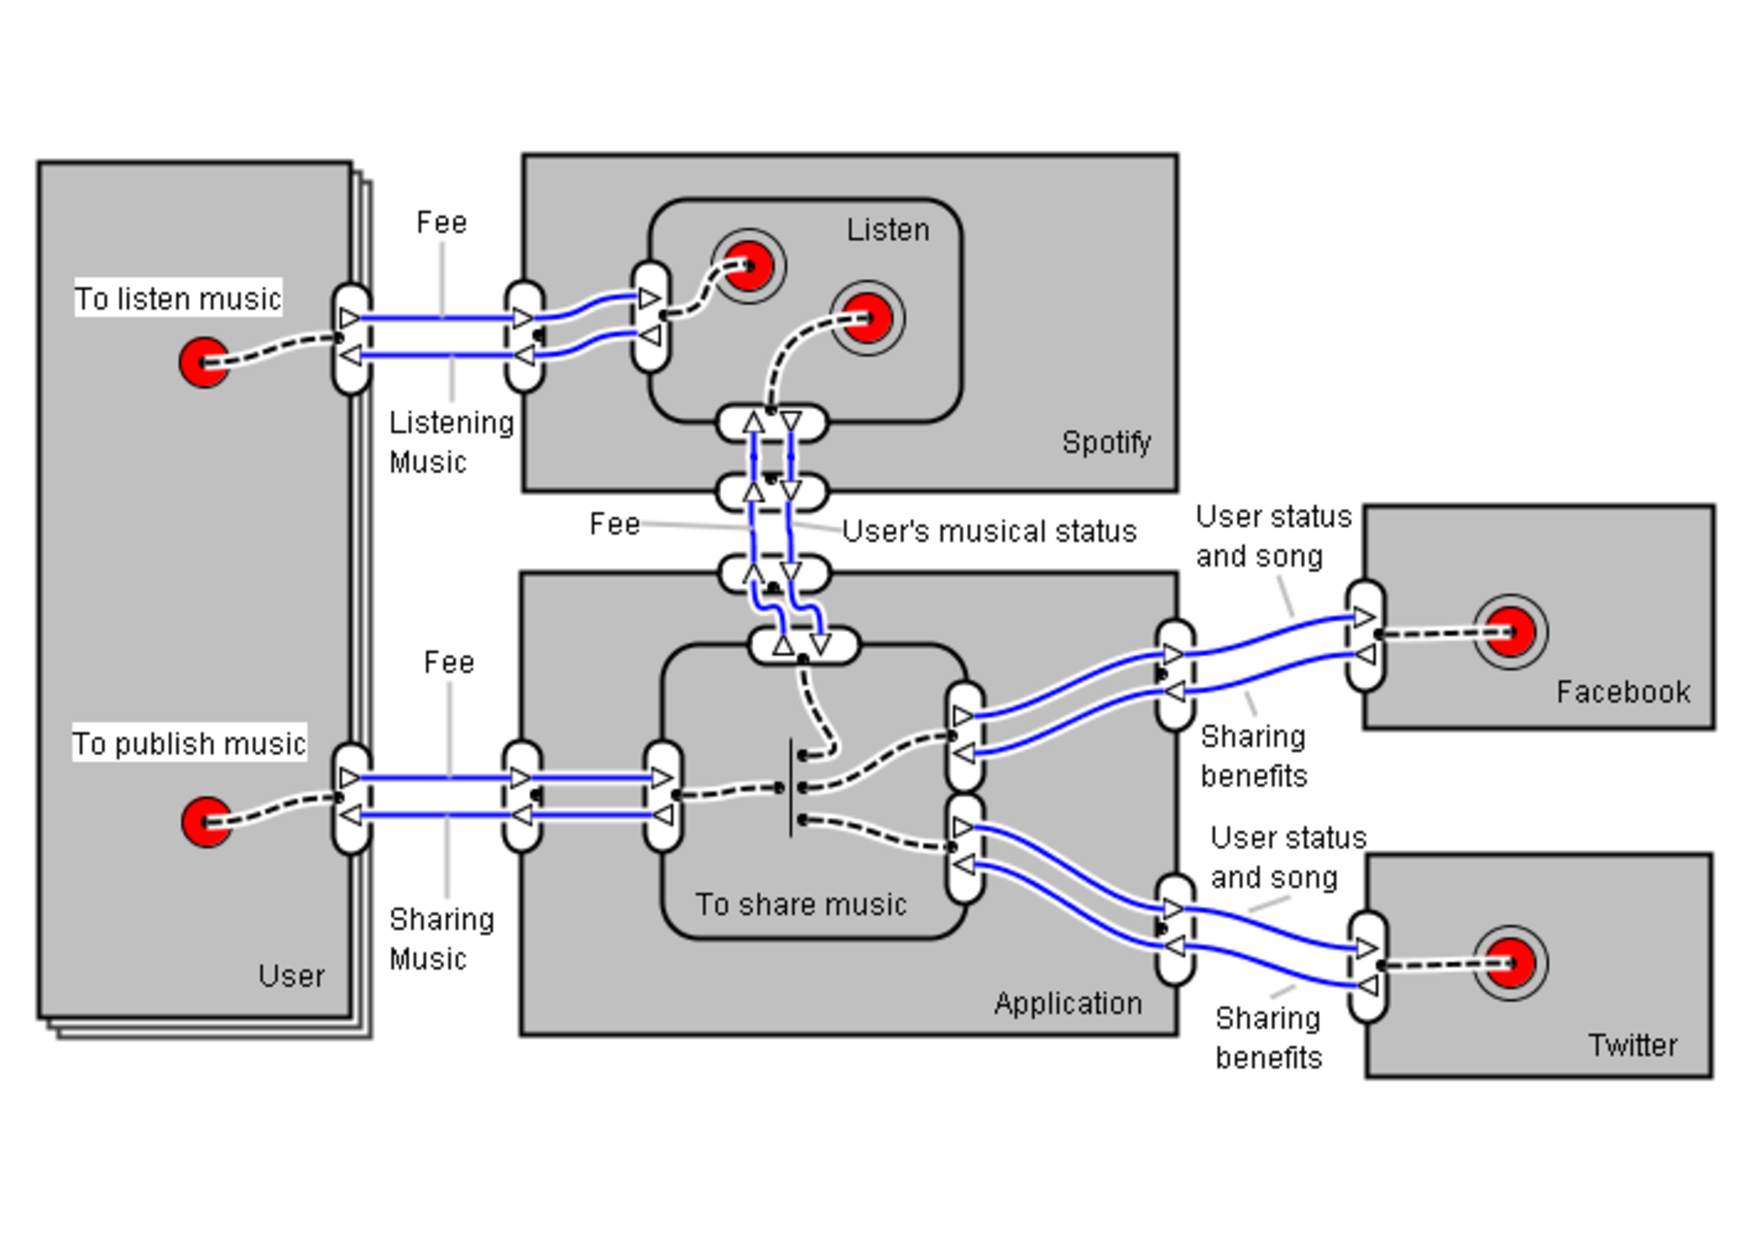
\includegraphics[width=0.70\textwidth]{figs/e3value}
\caption{E3value model of the "To Publish Music" scenario} 
\label{fig:E3valuemodel}
\end{figure}

Consider for instance the following scenario. A programmer wants to develop the application "To Publish Music" that monitors the music a person is listening during some periods of time and sends the song title  to Twitter and Facebook.  Social network users will have their status synchronized in  Twitter and Facebook  with the title of the music they are listening in Spotify.
For developing this application the programmer has to coordinate the calls to the methods offered by the following services:
\begin{itemize}
\item Music Services like  Spotify export methods for obtaining information  about the music a given user is listening:
\begin{itemize} \item {\sf\small get-Last-Song ( userid ): String} ; \end{itemize}
\item Facebook and Twitter services export methods for getting and updating the status of a given user: 
\begin{itemize} \item{\sf\small get-Status ( usedid ): String ; \item update-Status ( userid, new-status ): String}; \end{itemize}
%\item Mood Service exports a method for retrieving the mood of a  user: 
%\begin{itemize} \item{\sf\small get-Mood ( userid ): String} ;\end{itemize}
%It is a complex process that uses a log of the music listened by the user in Spotify during some period of time, and then according to the classification of each song it will determine her mood.
\end{itemize}

%


Figure \ref{fig:E3valuemodel} shows the E3 value model \cite{e3value} of 
the scenario. The model shows  Spotify and a private application (which is also a service) that directly interact with users for providing free services for listening and publish in information about music being listened by users. The private application   interacts with Spotify  for obtaining free information about the flow of music being listened by a user. Finally, the private application interacts with Facebook and Twitter for updating the user's status and thereby they share non material benefits (i.e., the fact that users subscribe to their networks and are active on them thanks to the private application).  

The "To Publish Music" scenario 
starts by contacting the music service Spotify for retrieving the user's  musical status. This information is sent to the mood service in order to calculate the mood of the user. Therefore, the Twitter and Facebook services are called for retrieving the status of the user.
%which is compared with other analysis data in order to determine the mood.  
Finally, Twitter and Facebook services are contacted in parallel for updating the user's status with the corresponding song. 

Besides the service composition that represents the order in which the services are called for implementing the application "To Publish Music" it is necessary to model the other constraints that represent the (i) conditions imposed by services for being contacted, for example the fact the Facebook and Twitter require authentication protocol in order to call their methods for updating the wall; (ii) the conditions stemming from the business rules of the application logic, for example the fact that the walls in Facebook and Twitter must show the same song title and if this is not possible then none of them is updated. This paper proposes the $\pi$-SOD-M method \cite{decastro1,decastro2}  for building applications by   modeling the application logic and its associated non-functional constraints and thereby ensuring the generation of reliable services' composition. This method is described in the following sections. 

%*********************************************************************************************************
\section{Modeling reliable services' compositions with $\pi$-SOD-M}\label{sec:sodm}
%*********************************************************************************************************
\begin{figure} [htpb]       
\centering  
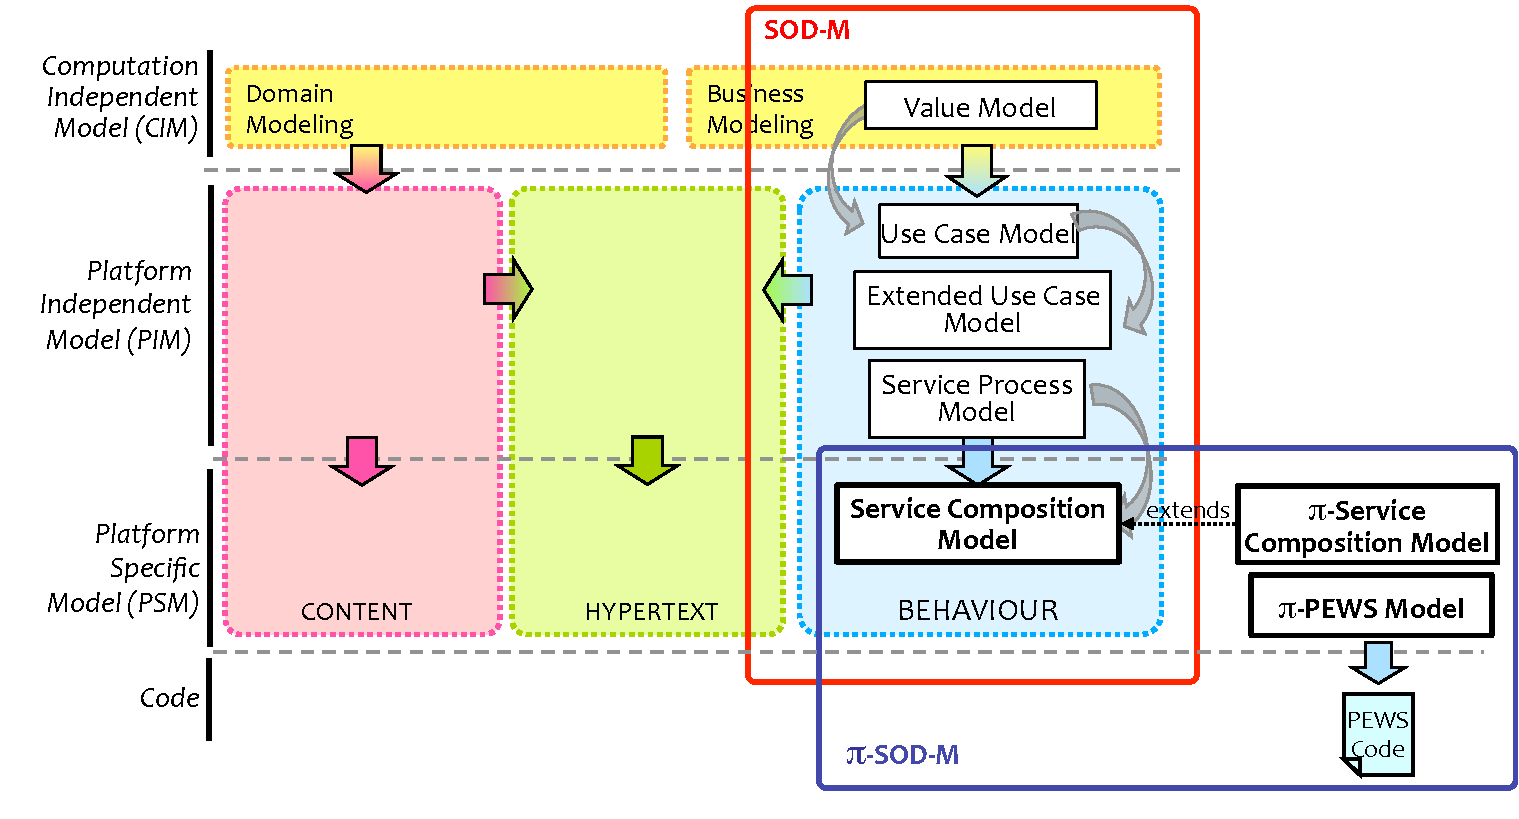
\includegraphics[width=0.65\textwidth]{figs/SODM}
\caption{SOD-M development process} 
\label{fig:sodm}
\end{figure}
SOD-M (see Figure \ref{fig:servicecompositionmodel}) defines a service-oriented approach that  provides  a set of guidelines to build IS based exclusively on services  \cite{decastro1,decastro2}.  Therefore, SOD-M proposes to use services as first-class objects for the whole process of the IS development and it  follows a MDA-based approach.
SOD-M proposes a set of models, extending from the highest level of abstraction of the MDA:  i) the three different MDA abstraction levels: CIM, PIM and PSM; and ii) SOD-M views: business and information system views. As shown in Figure \ref{fig:sodm}, the SOD-M model-driven process begins by building the high-level computational independent models and enables specific models for a service platform to be obtained as a result  \cite{decastro3}. For the sake of simplicity, in this work we  focus on the service composition model of SOD-M (highlighted in Figure  \ref{fig:sodm}) that we extended for considering non-functional properties. 


Our work  extends the  composition model of the PIM layer of the SOD-M method \cite{decastro1} with the notion of {\sf\small A-Policy} for representing service composition constraints \cite{Espinosa-Oviedo2011a}.  It  defines the $\pi$-{\sc Pews} \cite{Placido2010LTPD} meta-model providing guidelines for expressing the services composition and the policies, and also defines  Model to model transformation rules for generating  the implementation of reliable services' compositions implementations. Finally, our work defines model to text transformation rules for generating the  program that implements both the services' composition and the associated policies and that is executed by an adapted engine.

%..--..--..--..--..--..--..--..--..--..--..--..--..--..--..--..--..--..--..--..--..--..--..--..--..--..--..--..--..--..--..--..--..--..--..--..--..--..--
\subsection{$\pi$ service composition meta-model}
%..--..--..--..--..--..--..--..--..--..--..--..--..--..--..--..--..--..--..--..--..--..--..--..--..--..--..--..--..--..--..--..--..--..--..--..--..--..--

The policy  service composition meta-model ($\pi$-SCM)
represents the workflow needed to implement a business service by identifying {\sc Activities} and entities collaborating in the business processes (called {\sc Business Collaborators}) and performing them. An activity identified in the meta-model describes a fundamental behaviour unit which represents some transformation or processing in the system being modeled. There are two types of activities in this model: i) a Web Service (stereotyped as {\sc WS}); and ii) a simple operation not supported by a Web Service, called an Activity Operation (stereotyped as {\sc AOP}). Business collaborators are displayed in this model as a partition in the activity diagram. 
 \begin{figure}[htpb]       
\centering  
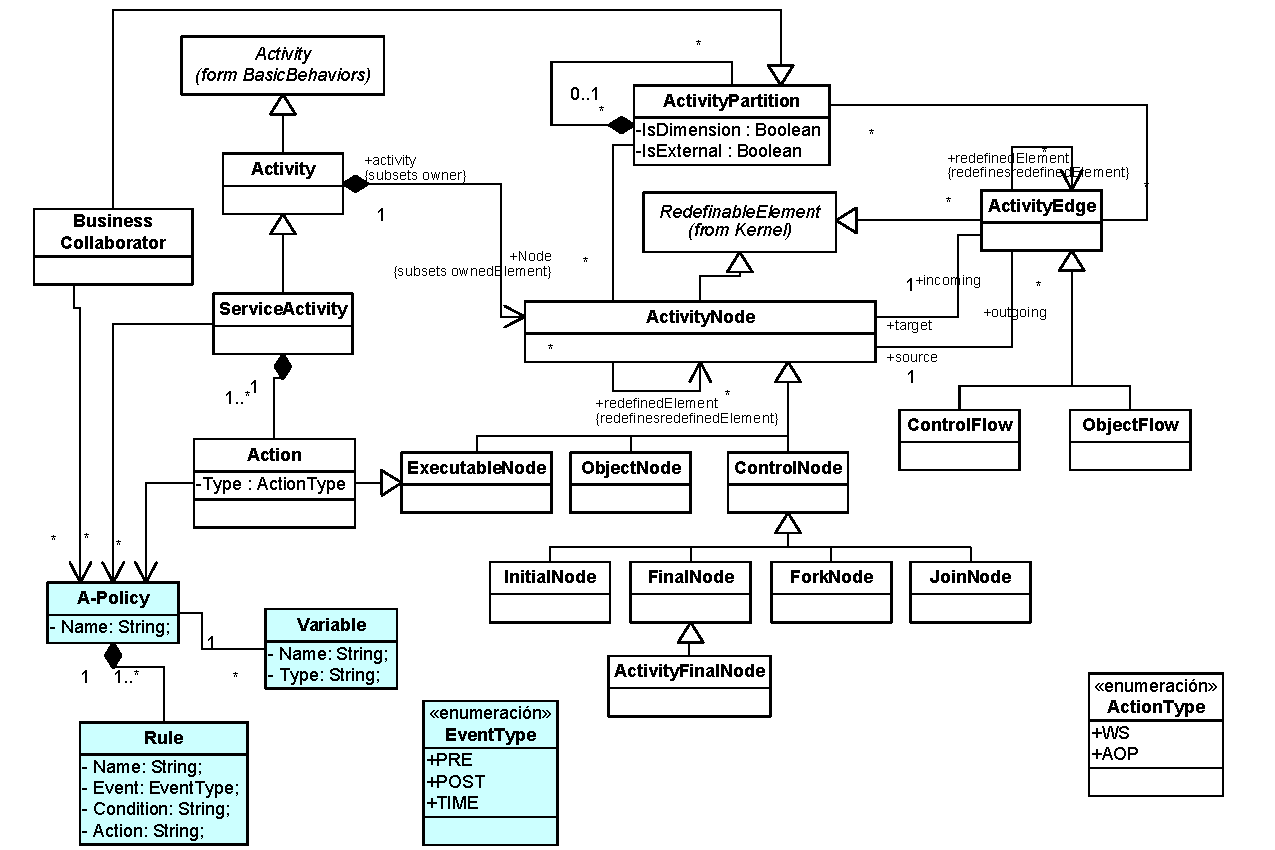
\includegraphics[width=0.80\textwidth]{figs/E-service-composition-metamodel}
\caption{Policy based service composition meta-model ($\pi$-SCM)} 
\label{fig:e-scomposition-metamodel}
\end{figure}

Instead of programming different  protocols within the application logic, we propose to include the modeling of non-functional constraints at the early stages of the service composition engineering process.  We model non-functional constraints of services compositions using the notion of {\em A-Policy} \cite{Espinosa-Oviedo2011a,CIC:eovszmc09b,CIC:eovszmc09c}, a kind of  pattern for specifying policy types. In order to represent constraints associated to services compositions, we  extended  the SOD-M service composition model with two concepts : {\sc Rule} and {\sc A-Policy} (see $\pi$-service composition model in Figure \ref{fig:e-scomposition-metamodel}). 

A {\sc Rule} represents the moment in which a constraint that must be evaluated (Event - Action) and the {\sc Action} to be executed for reinforcing  it. A {\sc Rule} can be associated to  activity boxes, to the control flow, message passing and to the compartments of the $\pi$-SCM. An A-policy type describes a specific constraint types that can correspond to non-functional constraints like   transactional behaviour, security and adaptability. An A-policy  defines a set of constraints over the execution states of the services� composition and defines strategies to enforce this property at the services� composition execution time.

An a-policy groups a set of rules that implement a non-functional constraint The a-policy expresses global variables and operations that can be shared by the rules and that can be used for expressing the condition and the condition parts.

 

\begin{figure}[htpb]         
\centering  
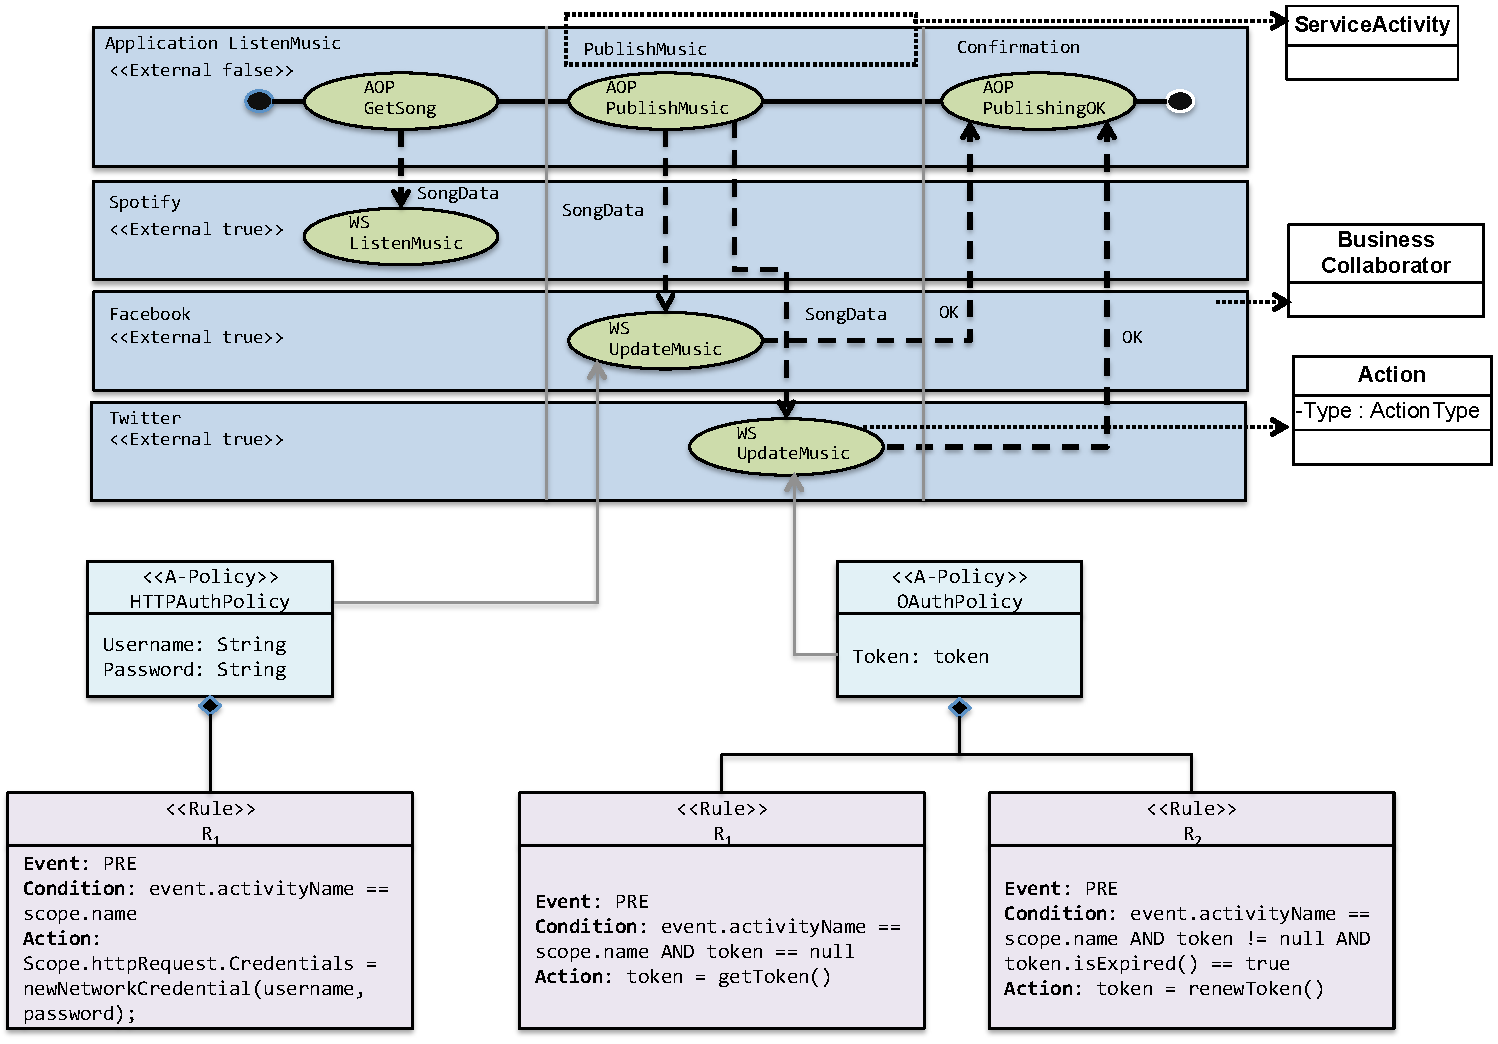
\includegraphics[width=0.70\textwidth]{figs/e-composition-model}
\caption{Service Composition Model for the business service To publish music} 
\label{fig:servicecompositionmodel}
\end{figure}

Figure \ref{fig:servicecompositionmodel} shows the $\pi$-SCM  that represents the composition process of the different activities needed to carry out the business service �To Publish Music�. There are three external business collaborators (Spotify, Twitter and Facebook). It also shows business process  of the  "To Publish Music" application that consists of three service activities. Note that in the service activity {\em PublishMusic} the service activity calls the activities of two service collaborators namely {\em Facebook} and {\em Twitter}.

Given that Facebook and Twitter services require authentication protocols in order to execute methods that will read and update the users' space. When these services are called  the call must be part of the authentication protocol required by these services.  
In the example we  associate two authentication policies, one for the open authentication protocol, represented by the class {\sc Twitter OAuthPolicy} that will be associated to the activity  {\sf\small UpdateTwitter} (see Figure \ref{fig:servicecompositionmodel}). In the same way, the  class {\sc Facebook HTTPAuthPolicy}, for the http authentication protocol will be associated to the activity {\sf\small UpdateFacebook}. 
 {\sf\small OAuth}  implements the open authentication protocol. 
As shown in Figure \ref{fig:servicecompositionmodel}, the a-policy  has a variable {\sf\small Token} that will be used to store the authentication token provided by the service. This variable type is imported through the library {\sf\small OAuth.Token}. The policy  defines two rules, both can be triggered by events of type {\sf\small ActivityPrepared}: (i) if no token has been associated to the variable {\sf\small token}, stated in by the condition of rule {\sf\small R$_1$}, then a token is obtained (action part of {\sf\small R$_1$}); (ii) if the token has expired, stated in the condition of rule {\sf\small R$_2$}, then it is renewed (action part of {\sf\small R$_2$}). Note that the code in the actions profits from the imported  {\sf\small OAuth.Token} for transparently obtaining or renewing a token from a third party.

{\sf\small HTTP-Auth} implements the HTTP-Auth protocol.  As shown in Figure  \ref{fig:servicecompositionmodel}, the policy imports an HTTP protocol library and it has two variables {\sf\small username} and {\sf\small password}.  The event of type {\sf\small ActivityPrepared} is the triggering event of the rule {\sf\small R$_1$}. On the notification of an event of that type, a credential is obtained using the username and password values. The object storing the credential is associated to the scope, i.e., the activity that will then use it for executing the method call.



Thanks to rules and policies  it is possible to model and associate non-functional properties to services' compositions  and then generate the code. For example, the atomic integration of information retrieved from different social network services, automatic generation of an integrated view of the operations executed in different social networks. Or for providing security in the communication channel when the payment service is called.

%..--..--..--..--..--..--..--..--..--..--..--..--..--..--..--..--..--..--..--..--..--..--..--..--..--..--..--..--..--..--..--..--..--..--..--..--..--..--
\subsection{$\pi$-{\sc Pews}  meta-model}\label{sec:pewsmetamodel}
%..--..--..--..--..--..--..--..--..--..--..--..--..--..--..--..--..--..--..--..--..--..--..--..--..--..--..--..--..--..--..--..--..--..--..--..--..--..--
The idea of the $\pi$-{\sc Pews} meta-model is based on the service composition approach provided by the language PEWS\cite{BaAM06} (\textit{Path Expressions for Web Services}), a programming language that lets the service designer  combine the methods or subprograms that
implement each operation of the service, in order to achieve the desired application logic. Figure \ref{fig:metamodel} presents the $\pi$-{\sc Pews} meta-model  
consisting of  classes representing :
\begin{itemize}
\item a service composition: {\sc Namespace} representing the interface exported by a service, {\sc Operation} that represents a call to a service method, {\sc CompositeOperation}, and  {\sc Operator} for representing a service composition and {\sc PewsExpression} representing a services' composition.
An expression can be an{\sc Operation} or a {\sc Compound Operation}, 
denoted by an identifier, the sequential ($\ . \ $) or parallel ($\ \| \ $) composition of services, 
the choice ($\ + \ $) among services, 
the sequential ($*$) or parallel ($\{\dots\}$) repetition of operation or the conditional execution of an operation ($[C]S$).

\item policies that can be associated to a service composition:  {\sc A-Policy}, {\sc Rule}, {\sc Event}, {\sc Condition}, {\sc Action}, {\sc State}, and {\sc Scope}.
\end{itemize}

\begin{figure}        
\centering  
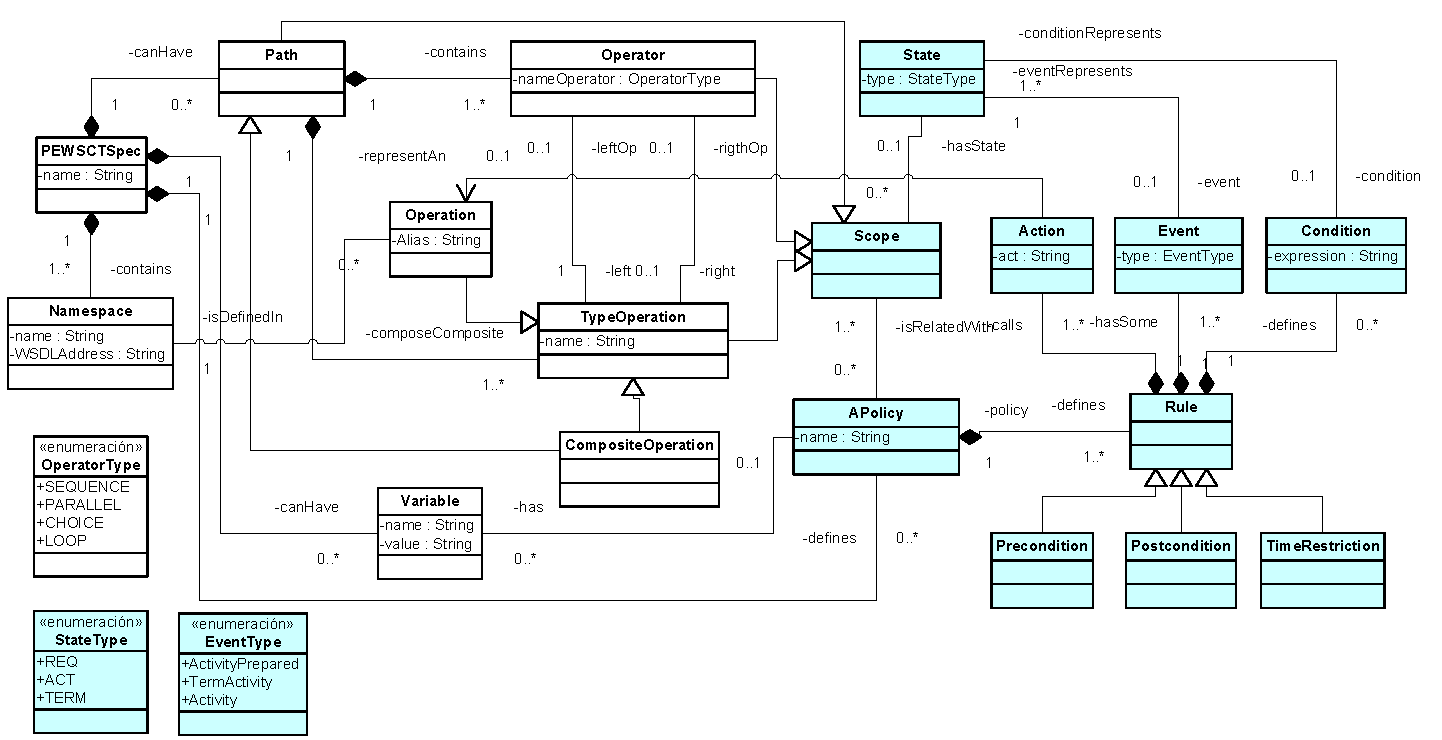
\includegraphics[width=0.80\textwidth]{figs/PEWSMetamodel}
\caption{$\pi$-{\sc Pews} Metamodel} 
\label{fig:metamodel}
\end{figure}

As shown in the diagram an {\sc A-Policy} is applied to a {\sc Scope} that can be either an {\sc Operation},  an {\sc Operator}, and a {\sc Path}.  It groups a set of ECA rules, each rule having a classic semantics, i.e, {\em when an event of type E occurs if  condition C is verified then execute the action A}.  Thus, an A-Policy represents a set of re-actions to be possibly executed if one or several triggering events of its rules are notified. 
\begin{itemize}
\item The class {\sc Scope} represents any element of a services' composition (i.e., operation, operator, path).

\item The class {\sc A-Policy} represents a recovery strategy implemented by ECA rules of the form {\sc Event} - {\sc Condition} - {\sc Action}. A policy has variables that represent the view of the execution state of its associated scope, that is required for executing the rules. The value of a variable is represented using the type Variable.
\end{itemize}
The class {\sc A-Policy} is specialized for defining specific constraints and  associating them a  to a concrete services� composition.


%
\begin{figure}[htpb]        
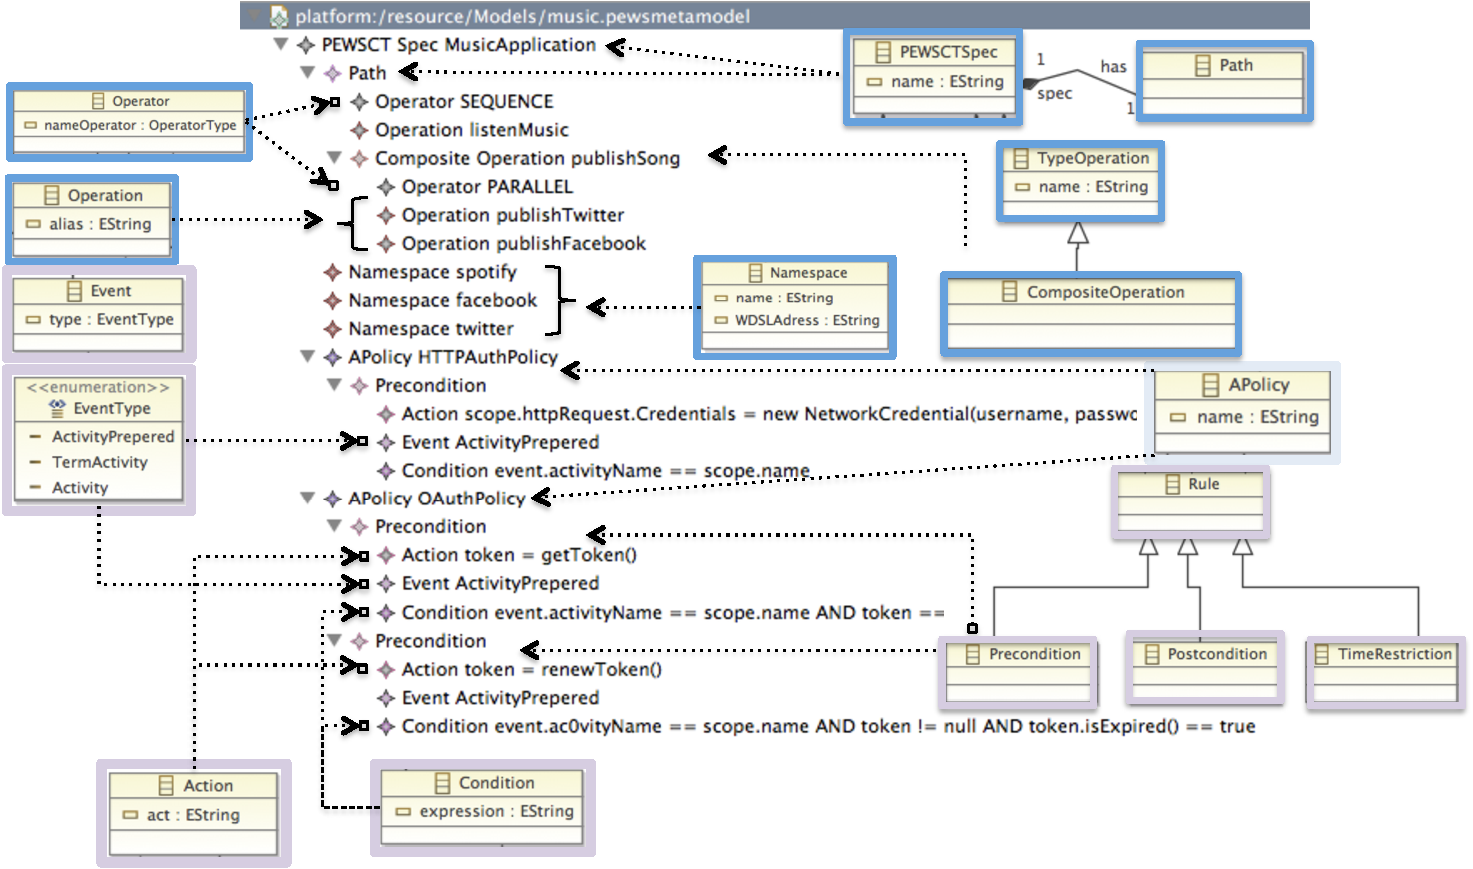
\includegraphics[width=0.80\textwidth]{figs/modeloPEWS}
\caption{$\pi$-{\sc Pews} generated model fo the "To Publish Music" application} 
\label{fig:p-scim}
\end{figure}
%
Figure \ref{fig:p-scim} shows the generated $\pi$-{\sc Pews} model for our example generated by the Eclipse plug-in that we implemented for this purpose. 
An authentication A-Policy represents the situation where an invocation in
an activity occurs until its sender and/or its recipient have been
identified. Typically, authentication A-Policies ensure that the invocation of the activity will be done within an authentication protocol. 

%..--..--..--..--..--..--..--..--..--..--..--..--..--..--..--..--..--..--..--..--..--..--..--..--..--..--..--..--..--..--..--..--..--..--..--..--..--..--
\subsection{Transformation rules}
%..--..--..--..--..--..--..--..--..--..--..--..--..--..--..--..--..--..--..--..--..--..--..--..--..--..--..--..--..--..--..--..--..--..--..--..--..--..--

Figure \ref{fig:transformations} shows the transformation principle between the elements of the $\pi$-SCM used for representing the service composition into the elements of the $\pi$-{\sc Pews} (see details of transformation rules in the appendix). There are two groups of rules: those that transform service composition elements of the $\pi$-SCM to $\pi$-{\sc Pews} elements; and those that transform rules grouped by policies into A-policy types. 

\begin{figure}    
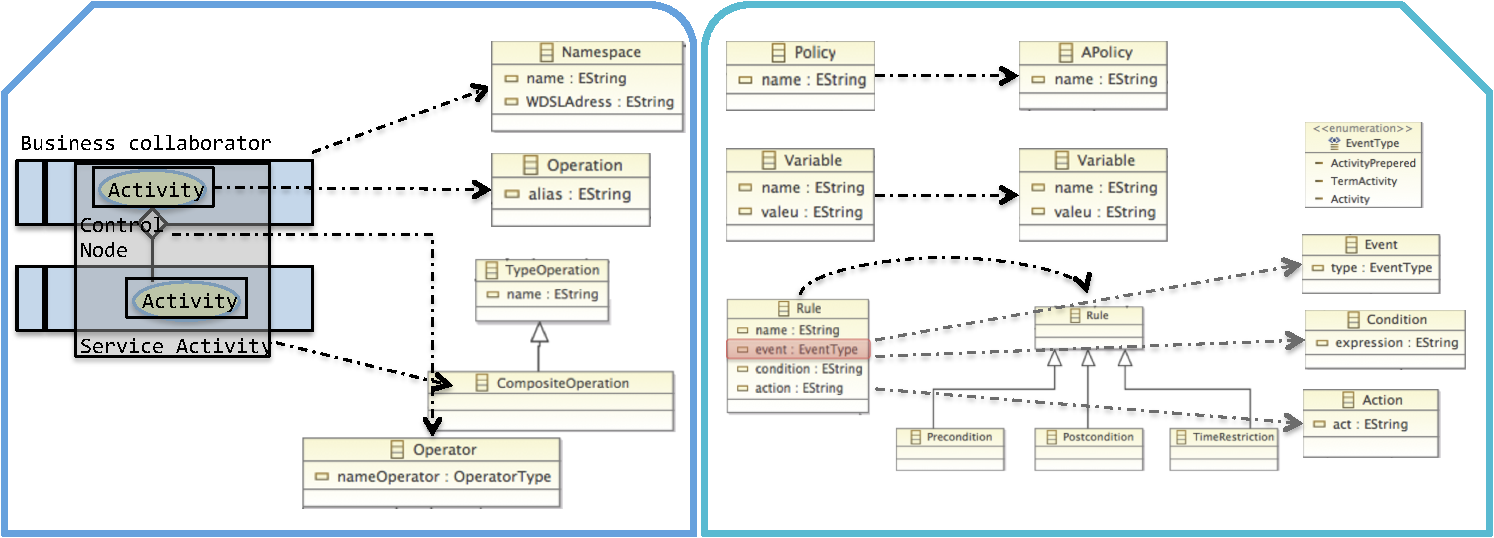
\includegraphics[width=0.95\textwidth]{figs/PI-SC-PI-P}
\caption{ $\pi$-SCM to $\pi$-{\sc Pews} transformation} 
\label{fig:transformations}
\end{figure}

% _ . _ . _ . _ . _ . _ . _ . _ . _ . _ . _ . _ . _ . _ . _ . _ . _ . _ .
\paragraph{First group of transformation rules:}
% _ . _ . _ . _ . _ . _ . _ . _ . _ . _ . _ . _ . _ . _ . _ . _ . _ . _ .
A named action of the $\pi$-SCM represented by  {\sc\em Action} and {\sc\em Action:name} is transformed to a class {\sc Operation} with a corresponding attribute name {\sc Operation:name}. A  named service activity represented by the elements {\sc\em ServiceActivity}  and  {\sc\em ServiceActivity:name} of the $\pi$-SCM, are  transformed into a named operation of the $\pi$-{\sc Pews} represented by the elements  {\sc Operation} and {\sc Operation:name}. When more than one actions are called, according to the following  composition patterns expressed using the operators {\sc\em merge, decision, fork and join} the transformations are (see Figure \ref{fig:mappingrules-2}) :
\begin{itemize}
\item   $op_1 . op_2$ if no {\sc\em ControlNode} is specified
\item $op_1 \parallel op_2 . op_3$ if control nodes of type {\sc\em fork, join} are combined 
 \item $op_1 + op_2 . op_3$ if control nodes of type {\sc\em decision, merge} are combined 
\end{itemize}

In the scenario "To Publish Music" the service activity {\sf PublishMusic} of the $\pi$-SC model specifies  calls to two {\sf Activitie}s of type {\em UpdateMusic}, respectively concerning the {\sf Business Service}s {\em Facebook} and {\em Twitter}. Given that no {\sf ConstrolNode} is specified by the $\pi$-SC model, the corresponding transformation is the expression that defines a {\sf Composite Operation} named {\em PublishSong} of the $\pi$-{\sc Pews} model of the form {\sf PublishFacebook} $\parallel$ {\sf PublishTwitter}.

% _ . _ . _ . _ . _ . _ . _ . _ . _ . _ . _ . _ . _ . _ . _ . _ . _ . _ .
\paragraph{Second group of transformation rules:}
% _ . _ . _ . _ . _ . _ . _ . _ . _ . _ . _ . _ . _ . _ . _ . _ . _ . _ .
The a-policies defined for the elements of the $\pi$-SCM are transformed into {\sc A-Policy} classes, named according to the names expressed in the source model. The transformation of the rules expressed in the $\pi$-SCM is guided by the event types associated to these rules.   The variables associated to a policy expressed in the$\pi$-SCM as {\sc\em $<$Variable:name, Variable:type$>$} are transformed into elements of type {\sc Variable} with attributes {\sc name} and {\sc type} directly specified from the elements {\sc\em  Variable:name} and {\sc\em Variable:type} of the $\pi$-SCM model.
As shown in Figure \ref{fig:mappingrules-1} of the Appendix, for an event of type {\sc\em Pre} the corresponding transformed rule is of type {\sc Precondition}; for an event of type {\sc\em Post} the corresponding transformed rule is of type {\sc Postcondition}; finally, for an event of type {\sc\em TimeRestriction} the corresponding transformed rule is of type {\sc Time}. The condition expression of a rule in the $\pi$-SCM ({\sc\em Rule:condition}) is transformed into a class {\sc\em Condition:expression} where the attributes of the expression are transformed into elements of type {\sc Attribute}.
The attribute event of a rule  ({\sc\em Rule:event}) in the $\pi$-SCM is transformed into an {\sc Event Type} according to the rule type. As shown in Figure \ref{fig:mappingrules-2} of the Appendix, the event type for a rule of type (i) {\sc Precondition} is {\sc ActivityPrepared}; (ii) {\sc Postcondition} is {\sc TermActivity}; (iii) {\sc TimeRestriction} is {\sc Temporal}. The {\sc\em Rule:Action} of a rule in the $\pi$-SCM is transformed into an {\sc Action:type}.

%
In the scenario "To Publish Music" the {\sf Policies} {\em OAuthPolicy} and {\em HTTPAuthPolicy} of the $\pi$-SCM model are transformed into policies of type {\sf Precondition} of the $\pi$-{\sc Pews} model of the scenario. Thus in both cases the events are of type {\sf ActivityPrepared}. These policies, as stated in the $\pi$-SCM model, are associated to {\sf Activities}. In the corresponding transformation they are associated to {\sf Operation}s {\em PublishFacebook} and {\em PublishTwitter}.

%*********************************************************************************************************
\section{Implementation issues}\label{sec:implementation}
%*********************************************************************************************************
\begin{figure}[htpb]
	\begin{center}
		\includegraphics[width=0.68\textwidth]{figs/Architecture.png}
	\end{center}
		\caption{General overview of the reliable service composition process}
   \label{fig:policymanager}
\end{figure}
This section  depicts the proposed process for generating reliable service compositions. For a given service based application, the process  consist in generating the  code starting from a $\pi$-SCM modeling an application. Note that the service composition model is not modeled from scratch at this level, but it is the result of a general process defined by the $\pi$-SOD-M method in which a set of models are built following a service oriented approach \cite{decastro1}.

To achieve the whole model transformation process, the Eclipse Modelling Framework (EMF) has been used. The EMF project is a modeling framework and code generation facility for building tools and other applications based on a structured data model. From a model specification described in XMI, EMF provides tools and runtime support to produce a set of Java classes for the model, along with a set of adapter classes that enable viewing and command-based editing of the model, and a basic editor. 

In order to automate the transformation we specify the transformation rules using ATL model transformation language \cite{11}. An ATL program is basically a set of rules that define how source model elements are matched and navigated to create and initialize the elements of the target models.
Finally, in order to generate code we have used Acceleo [http://www.acceleo.org/pages/home/en]. 
 
Figure \ref{fig:policymanager} depicts a general overview of the proposed process showing the set of plug-ins which have been developed in order to support the proposed framework:
\begin{itemize}
\item 	First, we  implemented using EMF, the meta-models  $\pi$- SCM and $\pi$-{\sc Pews}. After that, starting form these meta-models, we have developed the models plug-ins needed to support the graphical representation of the $\pi$- SCM and $\pi$-{\sc Pews} model ($\pi$-ServiceCompostion Model and $\pi$-PEWS Model plug-ins). 
\item	Then, we  developed using ATL, the mapping plug-in implementing the  mappings between models ($\pi$-ServiceComposition2$\pi$-PEWS Plug-in). 
\item 	Finally, we  created the code generation plug-in using Acceleo. To this end, the pews.mt program was codified including the entire model to text transformation needed to generate a  code starting form a $\pi$-PEWS model; and then a chain execution was created in order to execute the model to text transformation. 
\end{itemize}

As  shown in Figure \ref{fig:policymanager} , once an instance of a PEWS code is obtained starting form a particular $\pi$-service composition model it can be executed over policy based services' composition execution environment  consisting of a composition engine and a policy manager.  The  policy manager  consists of three main components Manager, for scheduling the execution of rules, C-Evaluator and A-Executor respectively for evaluating rules' conditions and executing their actions. The A-Policy Manager interacts with a composition engine thanks to a  message communication layer (MOM).

%Figure \ref{fig:policymanager} gives the global architecture of a policy based services' composition execution environment  consisting of a composition engine and a policy manager.
The composition engine manages the life cycle of the composition. Once a composition instance is activated, the engine schedules the composition activities according to the composition control flow. 
Each activity is seen as the process where the service method call is executed. 
The execution of an activity has four states: prepared, started, terminated, and failure. 
The execution of the control flow (sequence, and/or split and join) can also be prepared, started, terminated and raise a failure. 
%

At execution time, the evaluation of policies done by the policy manager must be synchronized with the execution of the service composition (i.e., the execution of an activity or a control flow).  Policies associated to a scope are activated when the execution of its scope starts. A policy will have to be executed only if one or several of its rules is triggered. If several rules are triggered the policy manager first builds an execution plan that specifies the order in which such rules will be executed according to the strategies defined in the following section. Once rules have been executed, the policy finishes its execution and returns to a sleeping state.
If rules belonging to several policies are triggered then policies are also ordered according to an execution plan. The order of policies has implications on the global order of the rules to be executed. 


We conducted an experimental validation of our approach  by implementing the "To Publish Music" application. Once the service composition model has been annotated with the corresponding policies, then the reliable composition code can be generated using the rules defined for this purpose. Our implementation includes a Java code generator that generates executable code for a reliable service composition. 
The model represents an services' composition expression and its associated policies. Figure \ref{fig:pewsexpression} shows the correspondence between the model and the statements that implement it, with a schematic representation of the business process. 
\begin{figure}        
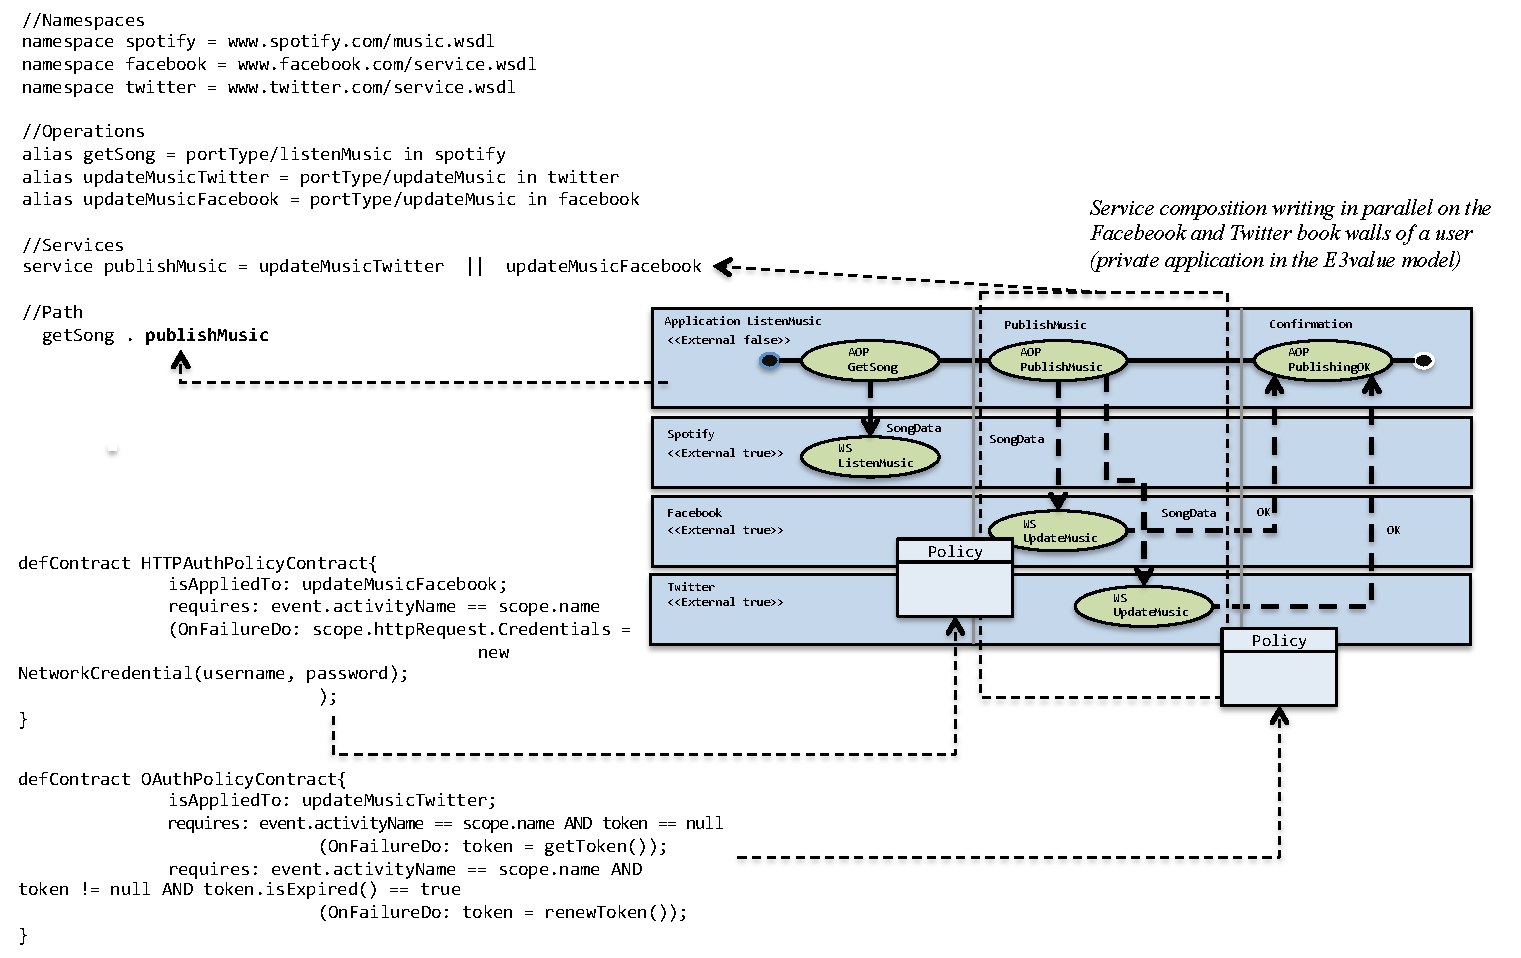
\includegraphics[width=0.85\textwidth]{figs/pews-expression}
\caption{Pews program implementing the "To Publish Music" application} 
\label{fig:pewsexpression}
\end{figure}
%*********************************************************************************************************
\section{Related works}\label{sec:related}
%*********************************************************************************************************
Current standards in services' composition implement functional, non-functional properties (NFP) and communication aspects by combining different languages and protocols. WSDL and SOAP among others are languages used respectively for describing services' interfaces and message exchange protocols for calling methods exported by such services. For adding a transactional behaviour to a services' composition it is necessary to implement WS-Coordination, WS-Transaction, WS-BussinessActivity and WS-AtomicTransaction. The selection of the adequate protocols for adding a specific NFP to a services' composition (e.g., security, transactional behaviour and adaptability) is responsibility of a programmer. As a consequence, the development of an application based on a services' composition is a complex and a time-consuming process. This is opposed to the philosophy of services that aims at facilitating the integration of distributed applications. 
Therefore, in contrast to these approaches, our work is inspired in the philosophy of \textit{separation of concerns} adopted in the construction of middleware for specifying policies to a services' composition in orthogonal way. 

There are few methodologies and approaches that address the explicit modeling  of non functional
properties for service based applications.   Software process methodologies for
building  services based applications have been proposed in\cite{PapazoglouH06,Papazoglou03,cdl2006,MilanovicM06,FeuerlichtM05,Ramollari_asurvey,somet2005}, and they focus mainly on the modeling and construction process of services based business processes that represent the application logic of information systems. 

 \textit{Design by Contract} \cite{HL05TACoS} is an approach for specifying web services and verifying them through runtime checkers before they are deployed. A contract adds behavioral information to a service specification, that is, it specifies the conditions in which methods exported by a service can be called. Contracts are expressed using the language \textit{jmlrac} \cite{LeavensCCRC02} . 
 

 The \textit{Contract Definition Language} (CDL) \cite{cdl2006} is a XML-based
description language, for defining contracts for services. There are an associated architecture framework, design standards and a methodology \cite{MilanovicM05,Milanovic05,Milanovic06,MilanovicM06}, for developing applications using services.  A services' based application  specification is generated after several 
B \cite{AbrialLNSS91} machines refinements that describe the services and their
compositions.

\cite{PapazoglouH06} proposes a methodology based on a SOA extension. This work defines a service
oriented business process development methodology with phases for business process development. The whole life-cycle is based on six phases: planning, analysis and design, construction and testing, provisioning, deployment, and execution and monitoring. 

IBM proposes a methodology for the development of SOA solutions, called SOMA \cite{soma}. SOMA defines a life-cycle with seven phases: business modeling and transformation, solution management, identification,
specification, realization, implementation and deployment monitoring and management.

 \cite{sommerville08} describes some key points for building services' based applications based on business process models that define the activities and information exchanged in a business processes. Activities in business process can be performed by services so that the model of business process
represents a composition of services. It classifies services   as public utilities, business services or
composition services. Software development that uses services involves creating programs for composing and configuring services to create new composite services. The service engineering process involves identifying services candidates, service interface and implementation definition, testing and deployment of each service.

Unlike the works presented, the main contribution of our proposal is the methodology description together with model representations in three levels (CIM, PIM and PSM)  for the design and development of distributed applications that can be reused and that are reliable. 

%*********************************************************************************************************
\section{Conclusions and future work}\label{sec:conclusions}
%*********************************************************************************************************
This paper presented $\pi$-SOD-M for specifying and designing reliable service based applications. We model and associate policies to  service based applications that represent both systems' cross-cutting aspects and use constraints stemming from the services used for implementing them.  We extended the SOD-M methodology, particularly the $\pi$-SCM (service composition meta-model) and $\pi$-{\sc Pews} meta-models for representing both the application logic and its associated non-functional constraints and then generating its executable code. We implemented the meta-models on the Eclipse platform and we validated the approach using a use case that uses authentication  policies. 

Non-functional constraints are related to business rules associated to the general "semantics" of the application and in the case of services' based applications, they also concern the use constraints imposed by the services. We are currently working on the definition of a methodology for explicitly expressing such properties in the early stages of the specification of services based applications. Having such business rules expressed and then translated and associated to the service composition can help to ensure that the resulting application is compliant to the user requirements and also to the characteristics of the services it uses.

Programming non-functional properties is not an easy task, so we are defining a set of predefined policy types with the associated use rules for guiding the programmer when she associates them to a concrete application. Policy type  that can also serve as patterns for programming or specializing the way non-functional properties are programmed.

\bibliographystyle{plain}
\bibliography{caise,S-Coord,Bib/e-commerce,Bib/trans,Bib/Component,Bib/XML,Bib/Workflow,Bib/SODM,Bib/G}



%*********************************************************************************************************
\section*{Appendix}\label{sec:appendix}
%*********************************************************************************************************
Figures \ref{fig:mappingrules-1},  \ref{fig:mappingrules-3}, \ref{fig:mappingrules-2} show the transformation rules between the $\pi$-SCM meta-model to the $\pi$-{\sc Pews}  meta-model. 
\begin{figure}        
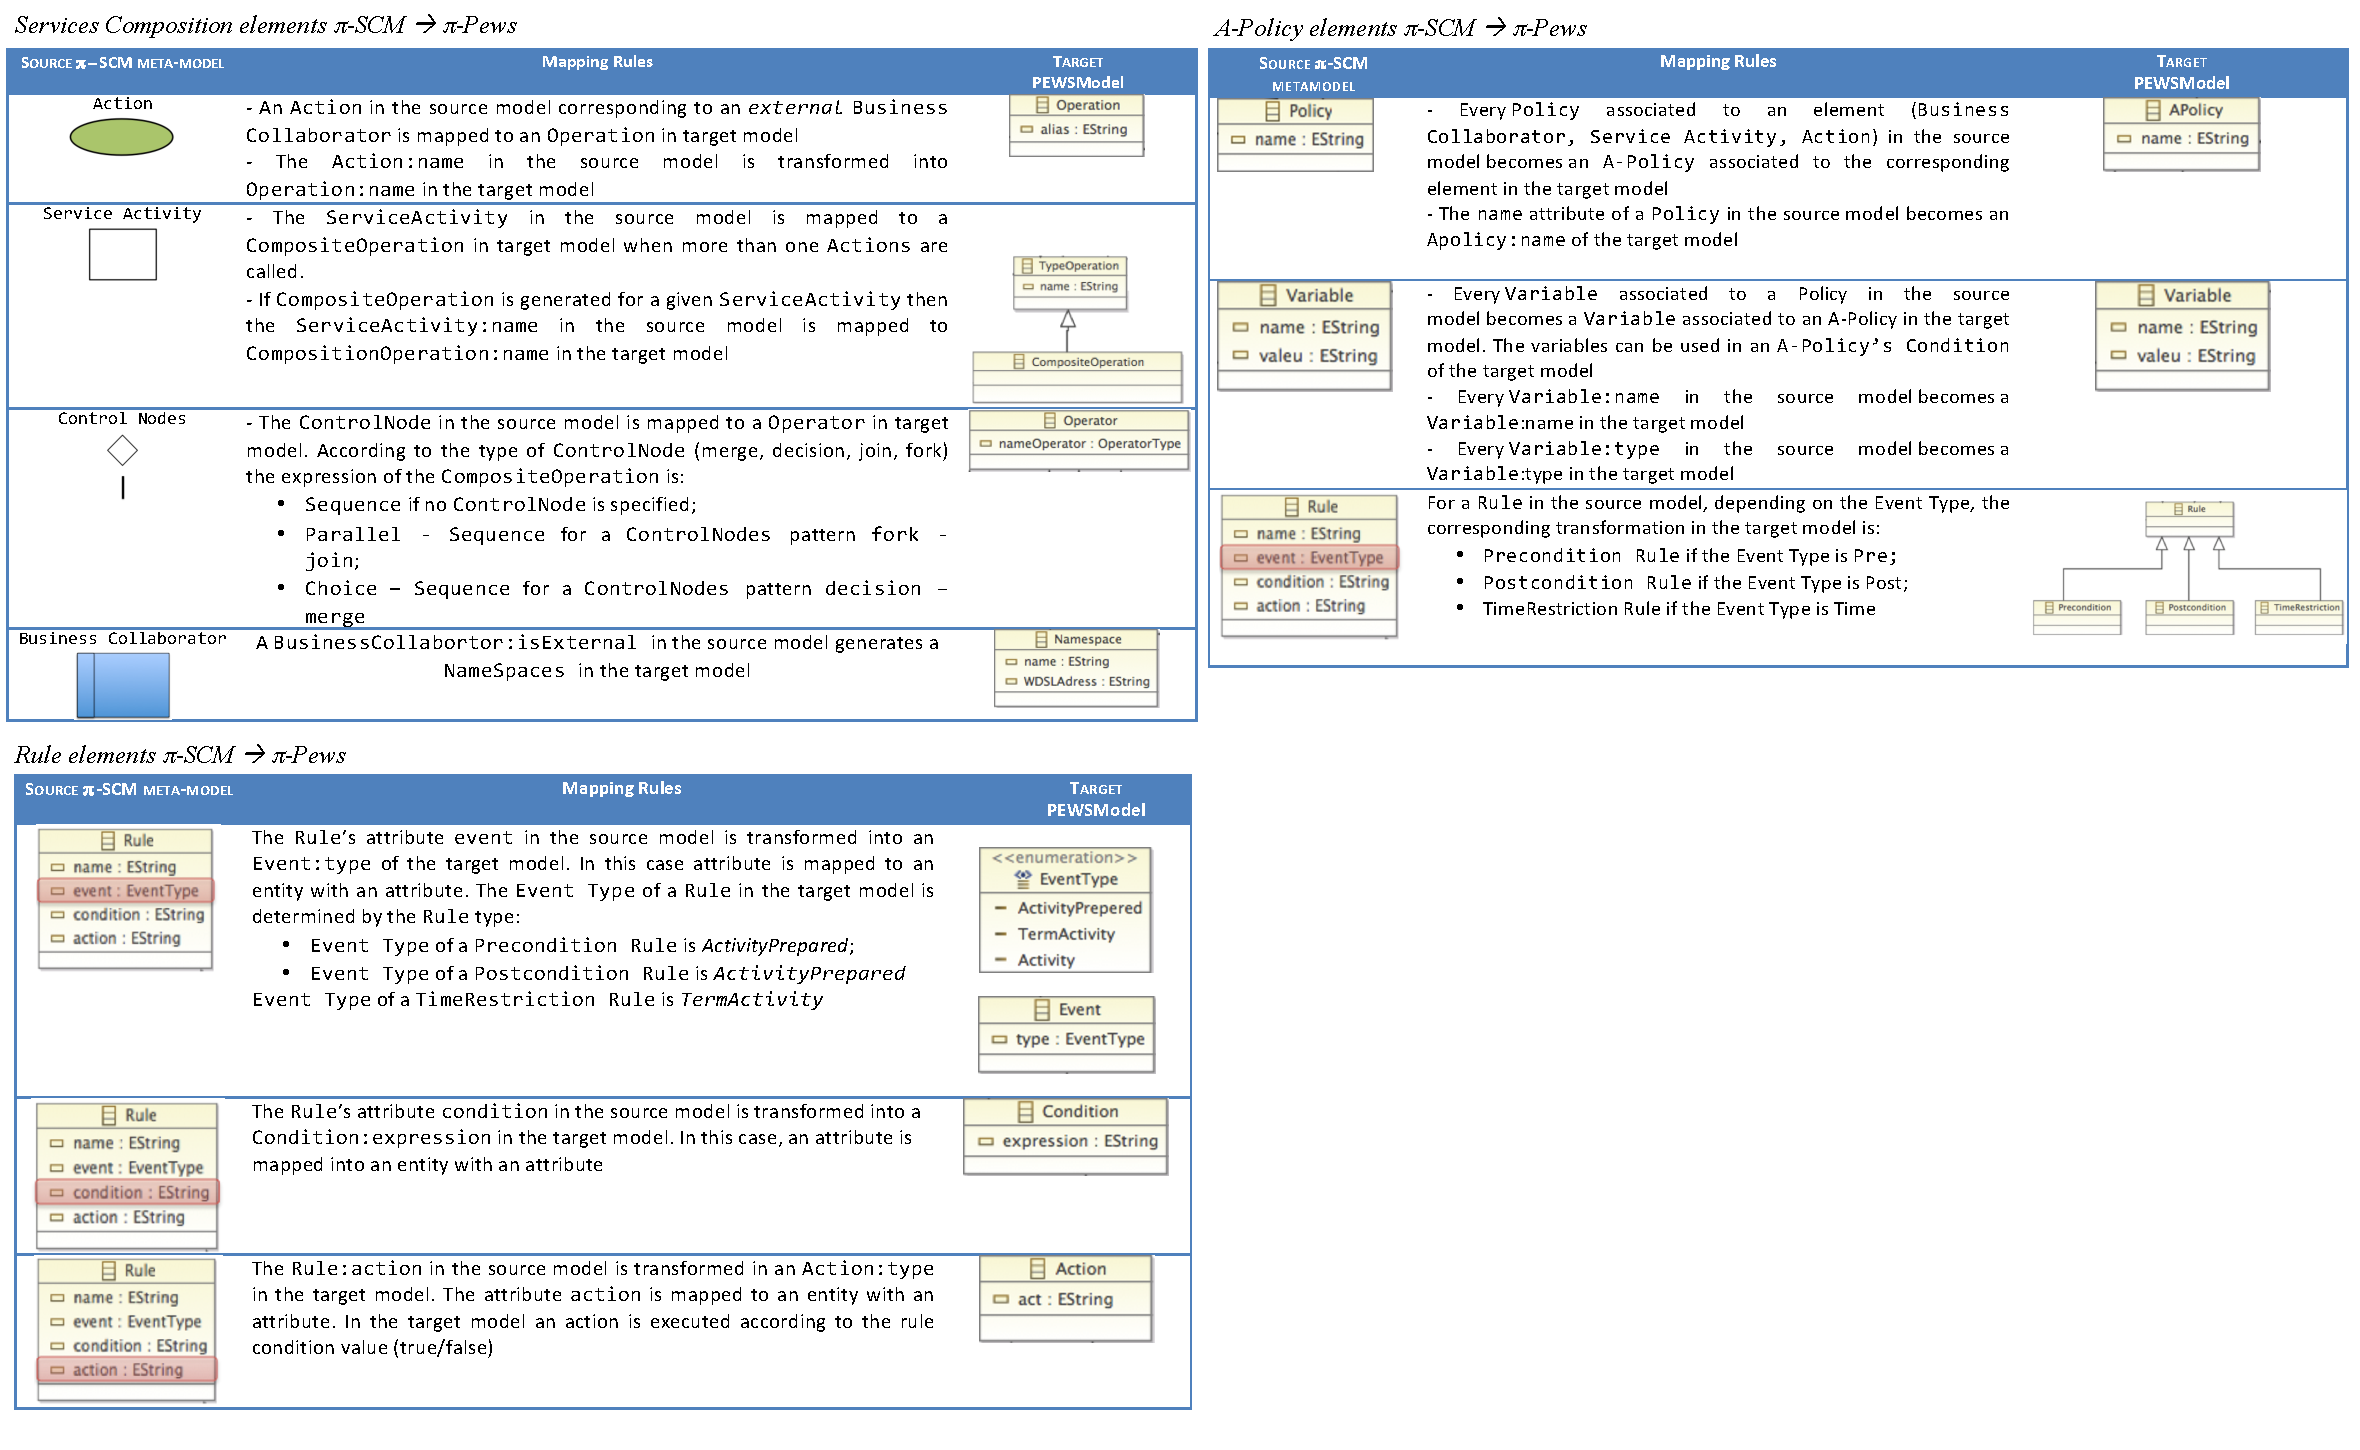
\includegraphics[width=0.75\textwidth]{figs/Mapping-1}
\caption{Mapping rules between service composition elements} 
\label{fig:mappingrules-1}
\end{figure}


\begin{figure}        
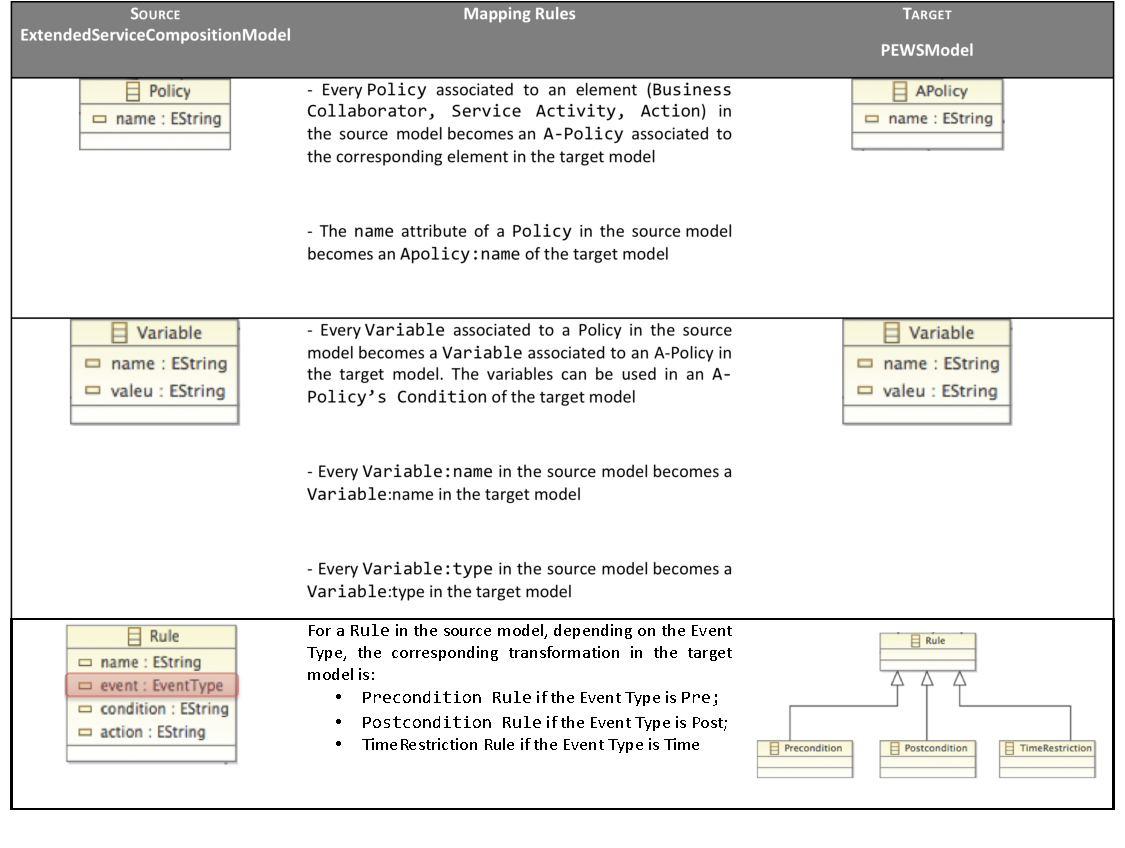
\includegraphics[width=0.75\textwidth]{figs/Mapping-3}
\caption{Mapping rules between $\pi$-SCM meta-model and $\pi$-{\sc Pews} policy elements} 
\label{fig:mappingrules-3}
\end{figure}


\begin{figure}        
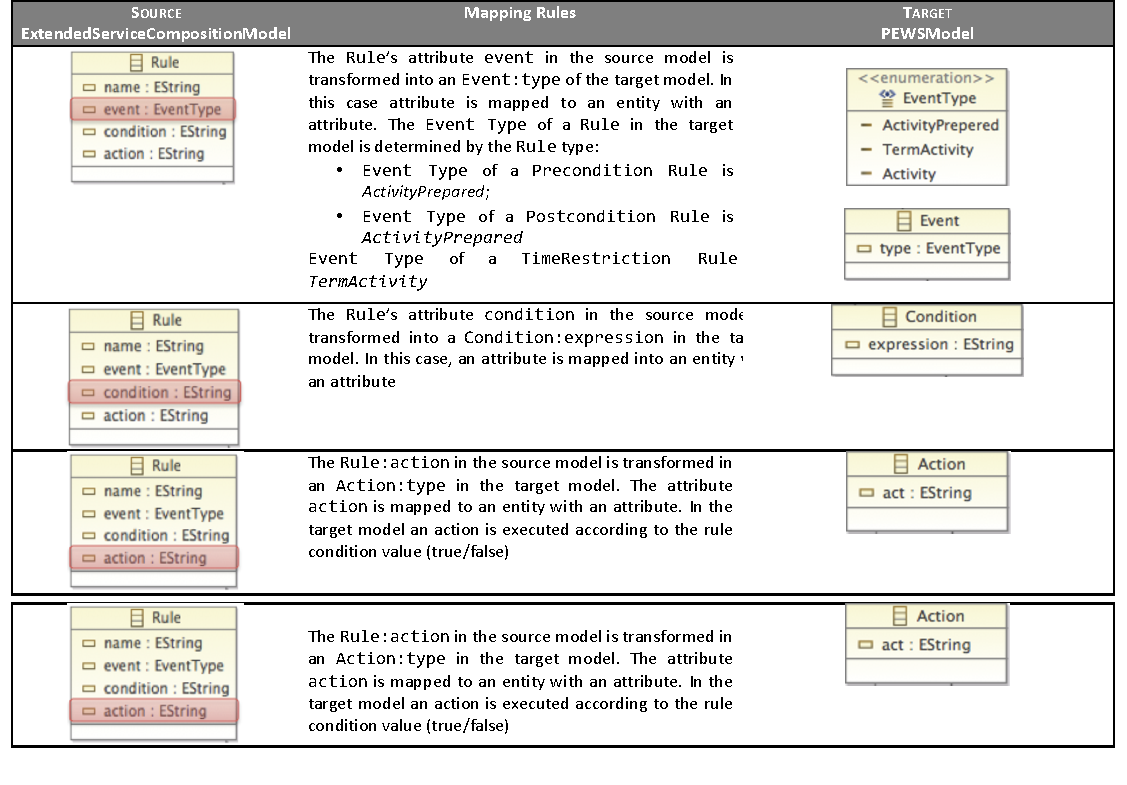
\includegraphics[width=0.75\textwidth]{figs/Mapping-2}
\caption{Mapping rules between $\pi$-SCM meta-model and $\pi$-{\sc Pews} rule elements} 
\label{fig:mappingrules-2}
\end{figure}



\end{document}
